% Options for packages loaded elsewhere
\PassOptionsToPackage{unicode}{hyperref}
\PassOptionsToPackage{hyphens}{url}
%
\documentclass[
]{article}
\title{Nuclear Energy: Kahan scale and Economic Political value scale}
\author{}
\date{\vspace{-2.5em}}

\usepackage{amsmath,amssymb}
\usepackage{lmodern}
\usepackage{iftex}
\ifPDFTeX
  \usepackage[T1]{fontenc}
  \usepackage[utf8]{inputenc}
  \usepackage{textcomp} % provide euro and other symbols
\else % if luatex or xetex
  \usepackage{unicode-math}
  \defaultfontfeatures{Scale=MatchLowercase}
  \defaultfontfeatures[\rmfamily]{Ligatures=TeX,Scale=1}
\fi
% Use upquote if available, for straight quotes in verbatim environments
\IfFileExists{upquote.sty}{\usepackage{upquote}}{}
\IfFileExists{microtype.sty}{% use microtype if available
  \usepackage[]{microtype}
  \UseMicrotypeSet[protrusion]{basicmath} % disable protrusion for tt fonts
}{}
\makeatletter
\@ifundefined{KOMAClassName}{% if non-KOMA class
  \IfFileExists{parskip.sty}{%
    \usepackage{parskip}
  }{% else
    \setlength{\parindent}{0pt}
    \setlength{\parskip}{6pt plus 2pt minus 1pt}}
}{% if KOMA class
  \KOMAoptions{parskip=half}}
\makeatother
\usepackage{xcolor}
\IfFileExists{xurl.sty}{\usepackage{xurl}}{} % add URL line breaks if available
\IfFileExists{bookmark.sty}{\usepackage{bookmark}}{\usepackage{hyperref}}
\hypersetup{
  pdftitle={Nuclear Energy: Kahan scale and Economic Political value scale},
  hidelinks,
  pdfcreator={LaTeX via pandoc}}
\urlstyle{same} % disable monospaced font for URLs
\usepackage[margin=1in]{geometry}
\usepackage{graphicx}
\makeatletter
\def\maxwidth{\ifdim\Gin@nat@width>\linewidth\linewidth\else\Gin@nat@width\fi}
\def\maxheight{\ifdim\Gin@nat@height>\textheight\textheight\else\Gin@nat@height\fi}
\makeatother
% Scale images if necessary, so that they will not overflow the page
% margins by default, and it is still possible to overwrite the defaults
% using explicit options in \includegraphics[width, height, ...]{}
\setkeys{Gin}{width=\maxwidth,height=\maxheight,keepaspectratio}
% Set default figure placement to htbp
\makeatletter
\def\fps@figure{htbp}
\makeatother
\setlength{\emergencystretch}{3em} % prevent overfull lines
\providecommand{\tightlist}{%
  \setlength{\itemsep}{0pt}\setlength{\parskip}{0pt}}
\setcounter{secnumdepth}{-\maxdimen} % remove section numbering
\usepackage{booktabs}
\usepackage{longtable}
\usepackage{array}
\usepackage{multirow}
\usepackage{wrapfig}
\usepackage{float}
\usepackage{colortbl}
\usepackage{pdflscape}
\usepackage{tabu}
\usepackage{threeparttable}
\usepackage{threeparttablex}
\usepackage[normalem]{ulem}
\usepackage{makecell}
\usepackage{xcolor}
\usepackage{multicol}
\usepackage{hhline}
\newlength\Oldarrayrulewidth
\newlength\Oldtabcolsep
\usepackage{hyperref}
\ifLuaTeX
  \usepackage{selnolig}  % disable illegal ligatures
\fi

\begin{document}
\maketitle

{
\setcounter{tocdepth}{2}
\tableofcontents
}
\newpage

\hypertarget{h1-nuclear-energy-will-be-seen-as-riskier-than-other-energy-technologies-in-india.}{%
\section{H1: Nuclear Energy will be seen as riskier than other energy
technologies in
India.}\label{h1-nuclear-energy-will-be-seen-as-riskier-than-other-energy-technologies-in-india.}}

\hypertarget{likert-responses-n-2160}{%
\subsection{Likert Responses (n= 2160)}\label{likert-responses-n-2160}}

The percentages are rounded off to whole numbers.

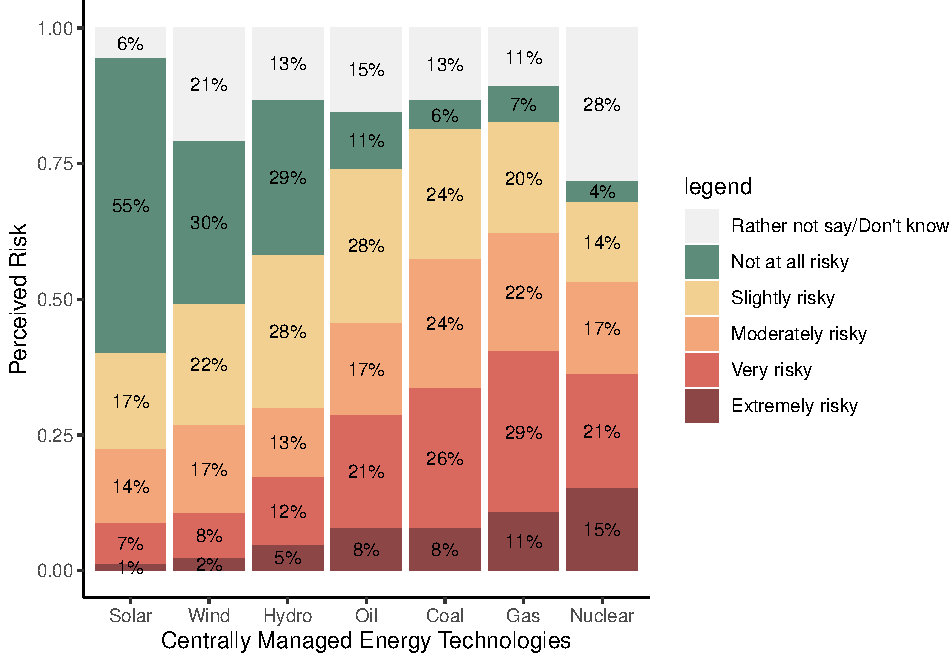
\includegraphics{Paper1_files/figure-latex/unnamed-chunk-5-1.pdf}
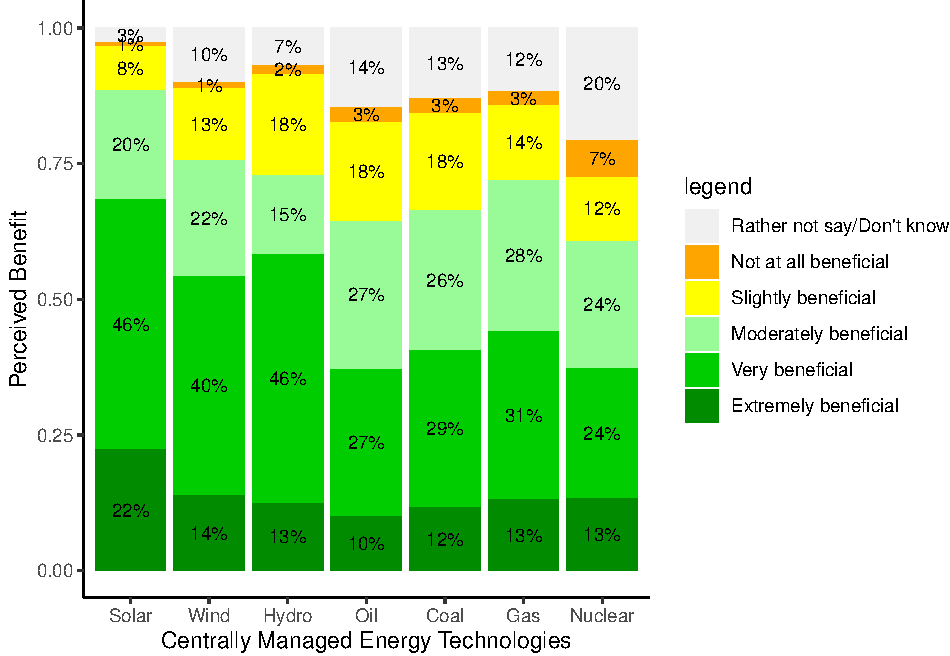
\includegraphics{Paper1_files/figure-latex/unnamed-chunk-5-2.pdf}

\newpage

\hypertarget{mean-perceived-risk-and-mean-perceived-benefit-for-all-energy-technologies.}{%
\subsection{Mean Perceived Risk and Mean Perceived Benefit for all
energy
technologies.}\label{mean-perceived-risk-and-mean-perceived-benefit-for-all-energy-technologies.}}

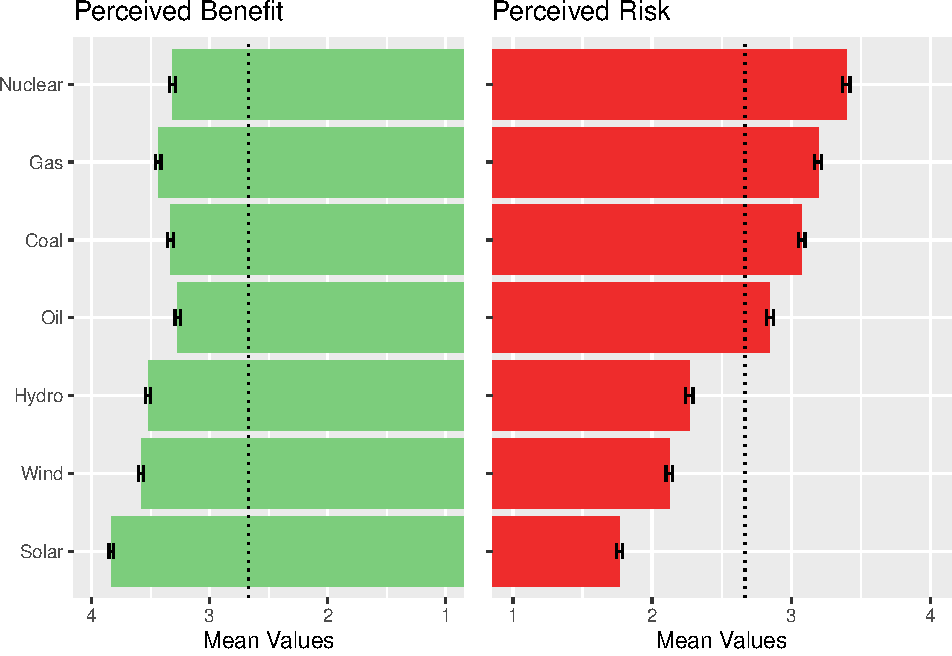
\includegraphics{Paper1_files/figure-latex/unnamed-chunk-7-1.pdf}

\hypertarget{boxplot-for-perceived-benefit-and-perceived-risk-by-technology}{%
\subsection{Boxplot for perceived benefit and perceived risk by
technology}\label{boxplot-for-perceived-benefit-and-perceived-risk-by-technology}}

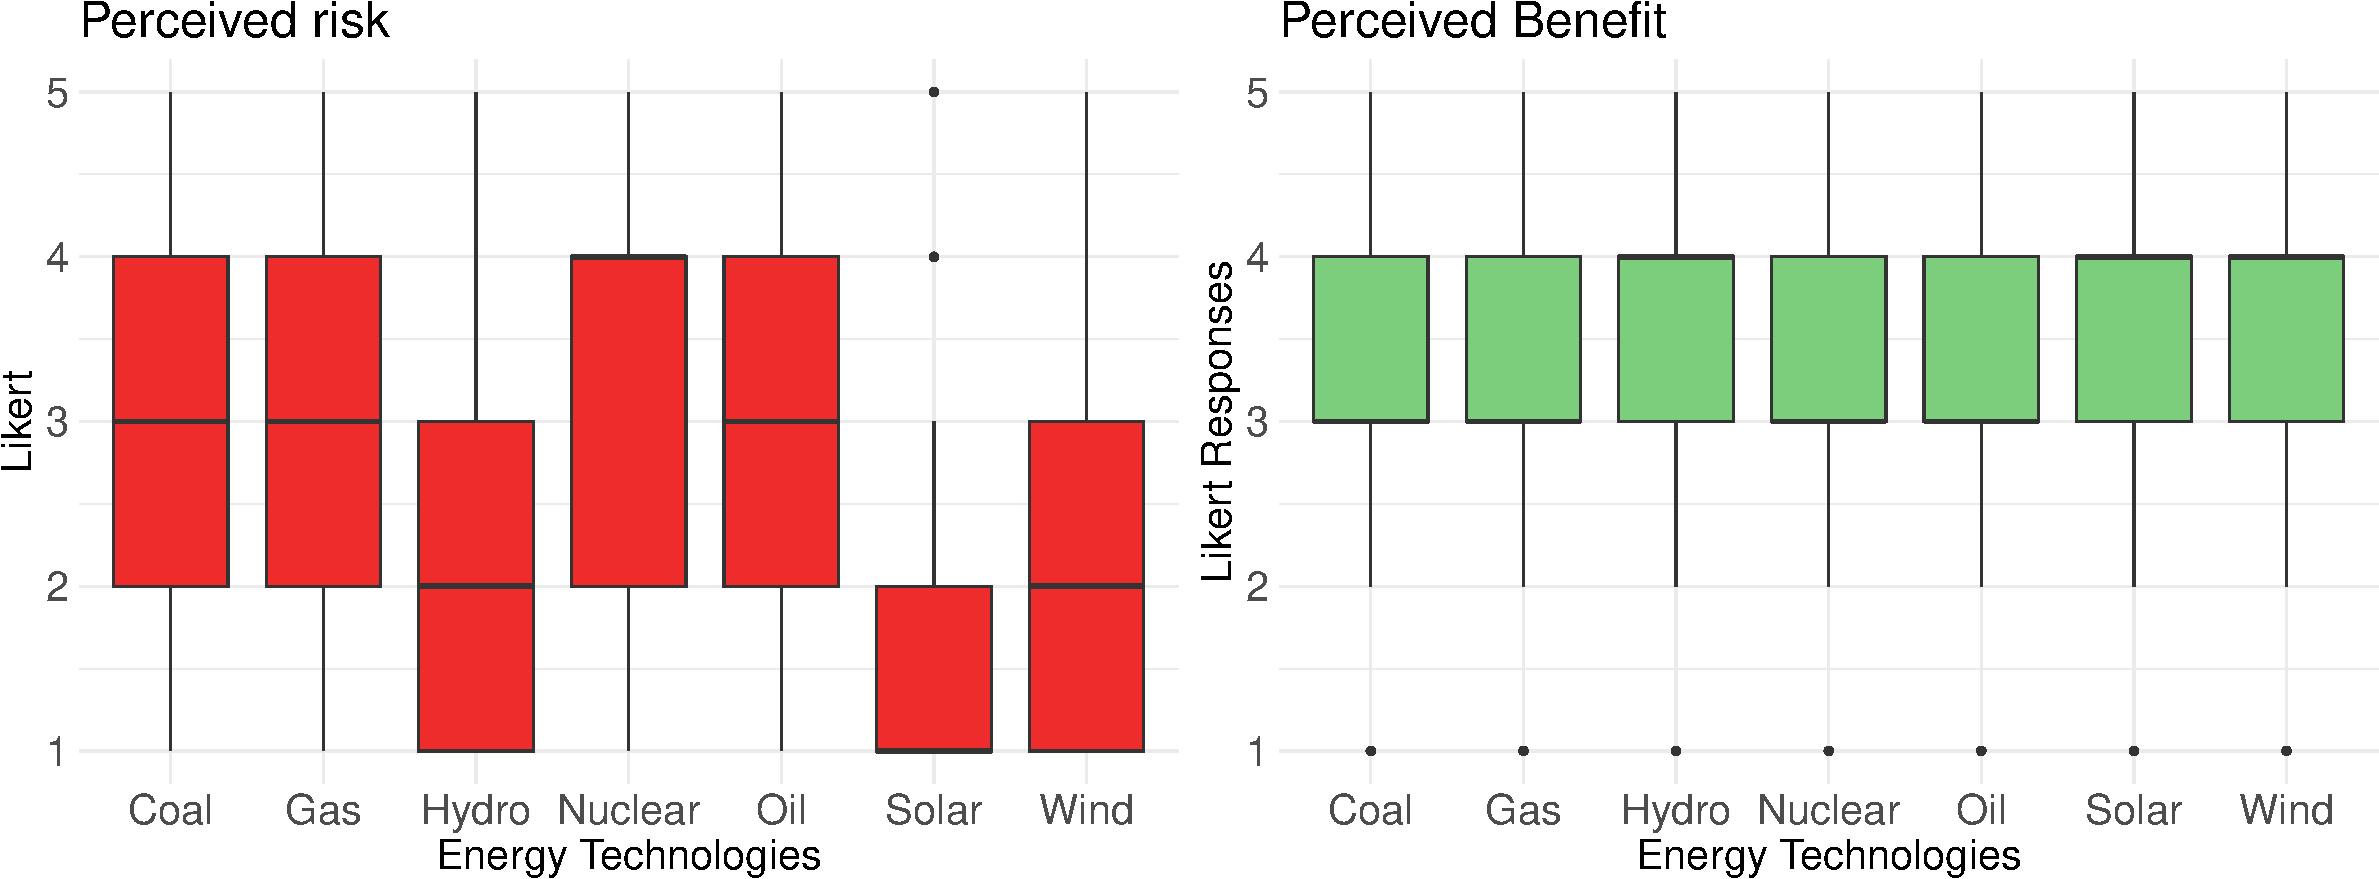
\includegraphics{Paper1_files/figure-latex/unnamed-chunk-8-1.pdf}

\newpage

\hypertarget{pairwise-t-test-mean-perceived-risk-and-mean-perceived-benefit-all-energy-technologies}{%
\subsection{Pairwise T-test: Mean perceived risk and mean perceived
benefit (all energy
technologies)}\label{pairwise-t-test-mean-perceived-risk-and-mean-perceived-benefit-all-energy-technologies}}

The red and green pairs indicate that there is a statistically
significant difference between the means of the two groups. White and
grey indicate - no differences between the means of the two groups.

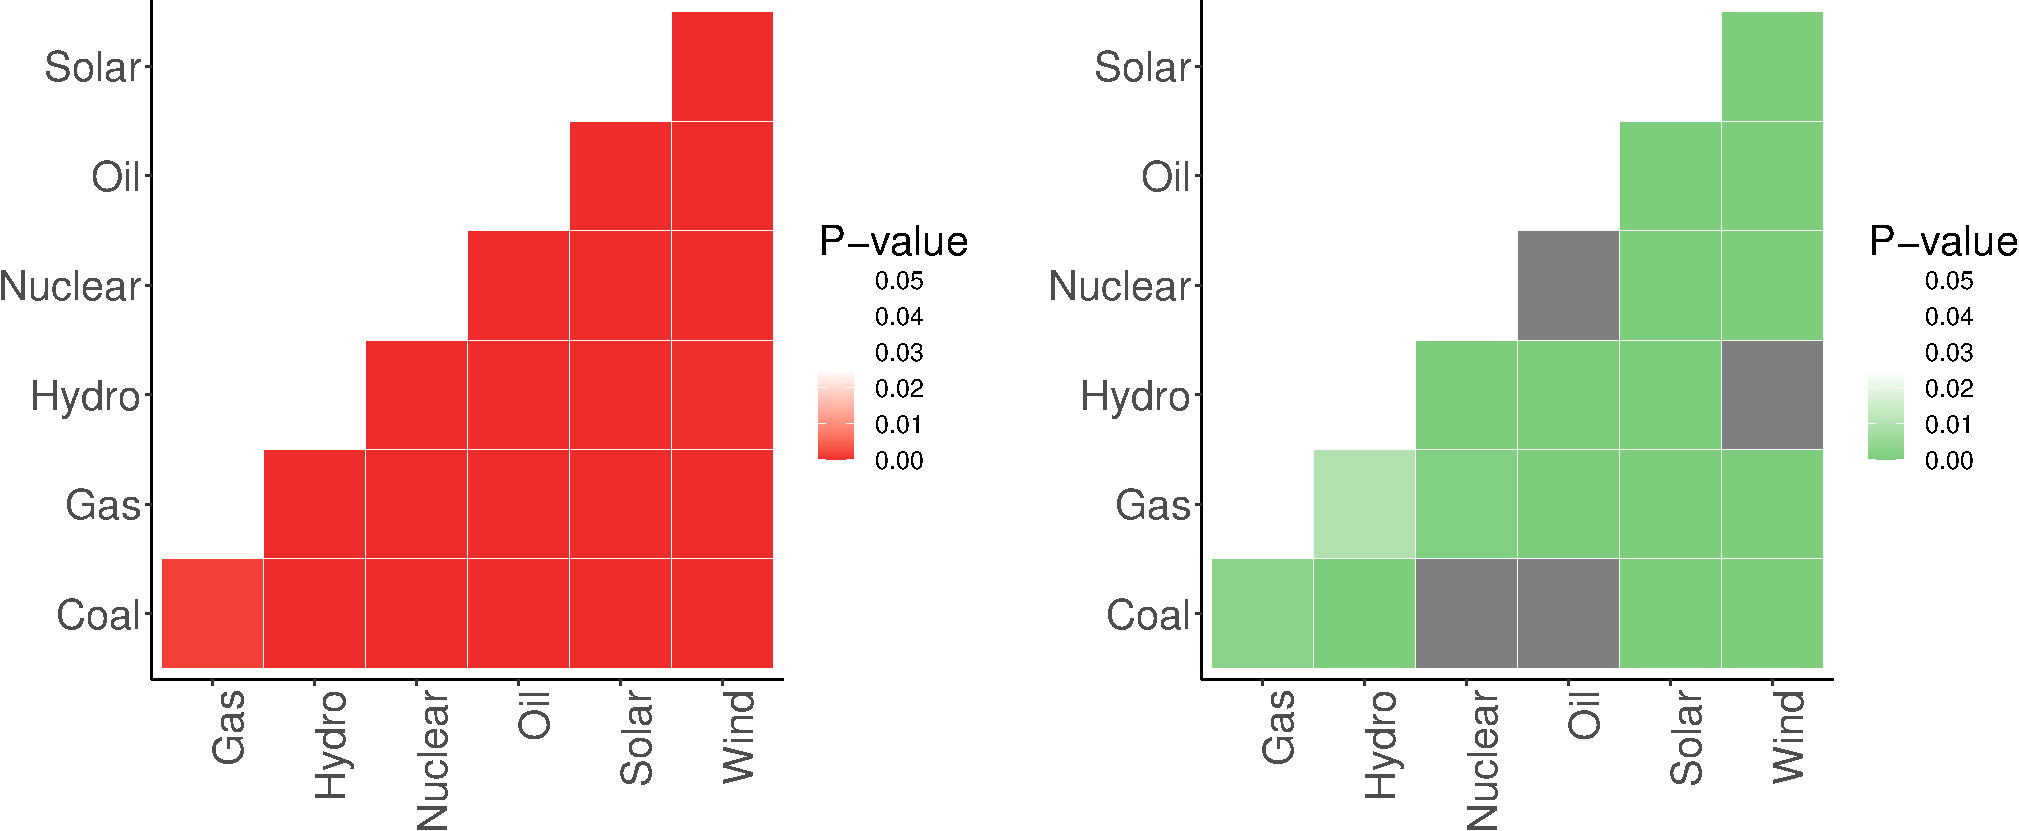
\includegraphics{Paper1_files/figure-latex/unnamed-chunk-9-1.pdf}

\newpage

\hypertarget{h2-gender-and-caste-will-have-significant-impact-like-gender-and-race-in-the-us-studies-of-risk.}{%
\section{H2: Gender and Caste will have significant impact like Gender
and Race in the US studies of
risk.}\label{h2-gender-and-caste-will-have-significant-impact-like-gender-and-race-in-the-us-studies-of-risk.}}

\hypertarget{two-linear-regression-models}{%
\subsection{two linear regression
models}\label{two-linear-regression-models}}

\begingroup\setlength{\tabcolsep}{1pt}\renewcommand{\arraystretch}{0.7}

\% Table created by stargazer v.5.2.3 by Marek Hlavac, Social Policy
Institute. E-mail: marek.hlavac at gmail.com \% Date and time: Mon, Sep
18, 2023 - 18:51:57

\begin{table}[!htbp] \centering 
  \caption{Results from 2 linear regression models} 
  \label{} 
\begin{tabular}{@{\extracolsep{5pt}}lcc} 
\\[-1.8ex]\hline 
\hline \\[-1.8ex] 
 & \multicolumn{2}{c}{\textit{Dependent variable:}} \\ 
\cline{2-3} 
\\[-1.8ex] & \multicolumn{2}{c}{Risky\_Nuclear} \\ 
\\[-1.8ex] & (1) & (2)\\ 
\hline \\[-1.8ex] 
 Uppercaste & 0.141$^{**}$ & $-$0.117$^{**}$ \\ 
  & (0.064) & (0.059) \\ 
  & & \\ 
 Male & 0.131$^{**}$ & 0.023 \\ 
  & (0.064) & (0.059) \\ 
  & & \\ 
 Hindu & $-$0.122 & $-$0.032 \\ 
  & (0.076) & (0.069) \\ 
  & & \\ 
 UrbanUrban & $-$0.082 & 0.081 \\ 
  & (0.063) & (0.064) \\ 
  & & \\ 
 age & 0.015 & $-$0.028 \\ 
  & (0.027) & (0.025) \\ 
  & & \\ 
 StateRajasthan &  & 0.245$^{***}$ \\ 
  &  & (0.093) \\ 
  & & \\ 
 StateTamil Nadu &  & $-$0.233$^{***}$ \\ 
  &  & (0.087) \\ 
  & & \\ 
 StateUttar Pradesh &  & $-$0.154 \\ 
  &  & (0.119) \\ 
  & & \\ 
 StateWest Bengal &  & 1.319$^{***}$ \\ 
  &  & (0.081) \\ 
  & & \\ 
 Constant & 3.360$^{***}$ & 3.209$^{***}$ \\ 
  & (0.104) & (0.096) \\ 
  & & \\ 
\hline \\[-1.8ex] 
Observations & 1,554 & 1,554 \\ 
R$^{2}$ & 0.011 & 0.215 \\ 
Adjusted R$^{2}$ & 0.007 & 0.210 \\ 
Residual Std. Error & 1.184 (df = 1548) & 1.056 (df = 1544) \\ 
F Statistic & 3.302$^{***}$ (df = 5; 1548) & 46.913$^{***}$ (df = 9; 1544) \\ 
\hline 
\hline \\[-1.8ex] 
\textit{Note:}  & \multicolumn{2}{r}{$^{*}$p$<$0.1; $^{**}$p$<$0.05; $^{***}$p$<$0.01} \\ 
\end{tabular} 
\end{table} 
\endgroup

\newpage

\hypertarget{h3-regional-differences-will-have-a-strong-impact}{%
\section{H3: Regional differences will have a strong
impact}\label{h3-regional-differences-will-have-a-strong-impact}}

\hypertarget{linear-regression-where-mean-value-is-the-intercept}{%
\subsection{Linear regression where Mean value is the
intercept}\label{linear-regression-where-mean-value-is-the-intercept}}

Same model with mean value as intercept.

\begingroup\setlength{\tabcolsep}{1pt}

\renewcommand{\arraystretch}{0.7}

\% Table created by stargazer v.5.2.3 by Marek Hlavac, Social Policy
Institute. E-mail: marek.hlavac at gmail.com \% Date and time: Mon, Sep
18, 2023 - 18:51:57

\begin{table}[!htbp] \centering 
  \caption{Results from 2 linear regression models} 
  \label{} 
\begin{tabular}{@{\extracolsep{5pt}}lcc} 
\\[-1.8ex]\hline 
\hline \\[-1.8ex] 
 & \multicolumn{2}{c}{\textit{Dependent variable:}} \\ 
\cline{2-3} 
\\[-1.8ex] & \multicolumn{2}{c}{Risky\_Nuclear} \\ 
\\[-1.8ex] & (1) & (2)\\ 
\hline \\[-1.8ex] 
 Uppercaste\_centered & 0.141$^{**}$ & $-$0.117$^{**}$ \\ 
  & (0.064) & (0.059) \\ 
  & & \\ 
 Male\_centered & 0.131$^{**}$ & 0.023 \\ 
  & (0.064) & (0.059) \\ 
  & & \\ 
 Hindu\_centered & $-$0.122 & $-$0.032 \\ 
  & (0.076) & (0.069) \\ 
  & & \\ 
 Urban\_centered & $-$0.082 & 0.081 \\ 
  & (0.063) & (0.064) \\ 
  & & \\ 
 age\_centered & 0.015 & $-$0.028 \\ 
  & (0.027) & (0.025) \\ 
  & & \\ 
 StateMaharashtra &  & $-$0.245$^{***}$ \\ 
  &  & (0.093) \\ 
  & & \\ 
 StateTamil Nadu &  & $-$0.479$^{***}$ \\ 
  &  & (0.099) \\ 
  & & \\ 
 StateUttar Pradesh &  & $-$0.400$^{***}$ \\ 
  &  & (0.122) \\ 
  & & \\ 
 StateWest Bengal &  & 1.074$^{***}$ \\ 
  &  & (0.092) \\ 
  & & \\ 
 Constant & 3.398$^{***}$ & 3.359$^{***}$ \\ 
  & (0.031) & (0.072) \\ 
  & & \\ 
\hline \\[-1.8ex] 
Observations & 1,554 & 1,554 \\ 
R$^{2}$ & 0.011 & 0.215 \\ 
Adjusted R$^{2}$ & 0.007 & 0.210 \\ 
Residual Std. Error & 1.184 (df = 1548) & 1.056 (df = 1544) \\ 
F Statistic & 3.302$^{***}$ (df = 5; 1548) & 46.913$^{***}$ (df = 9; 1544) \\ 
\hline 
\hline \\[-1.8ex] 
\textit{Note:}  & \multicolumn{2}{r}{$^{*}$p$<$0.1; $^{**}$p$<$0.05; $^{***}$p$<$0.01} \\ 
\end{tabular} 
\end{table} 
\endgroup

\newpage

\hypertarget{regional-differences-graph}{%
\subsection{Regional Differences
Graph}\label{regional-differences-graph}}

Following is a graph of z scores calculated from mean perceived risk
from nuclear energy by state.

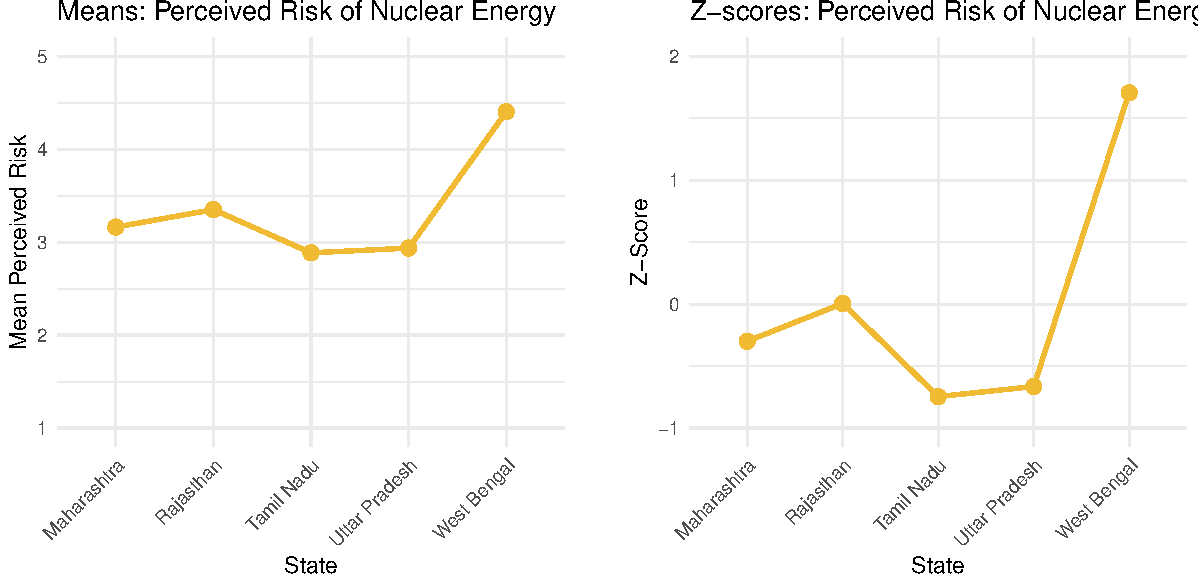
\includegraphics{Paper1_files/figure-latex/unnamed-chunk-15-1.pdf}

\newpage

\hypertarget{confirmatory-factor-analysiscfa-kahan-scale}{%
\section{Confirmatory Factor Analysis(CFA): Kahan
Scale}\label{confirmatory-factor-analysiscfa-kahan-scale}}

\textbf{Cronbach's Alpha on Kahan et al(2007) Scale: A Note}

The Individualism items (indicated by K\_I) were bringing down the
Cronbach's alpha values in the Kahan scale. The Alpha for Individualism-
Communitarian scale was 0.49. After removing the Individualism items
(K\_I) the alpha for this factor was 0.71. The reasons for this could be
that the individualism items are not well adapted to the Indian
population.

\begin{table}[!h]

\caption{\label{tab:unnamed-chunk-18}Fit Measures from the CFA}
\centering
\begin{tabular}[t]{lr}
\toprule
Measure & Value\\
\midrule
\cellcolor{gray!6}{Comparative Fit Index (CFI)} & \cellcolor{gray!6}{0.954}\\
Tucker-Lewis Index (TLI) & 0.925\\
\cellcolor{gray!6}{Root Mean Square Error of Approximation(RMSEA)} & \cellcolor{gray!6}{0.074}\\
RMSEA 90 Percent confidence interval - lower & 0.100\\
\cellcolor{gray!6}{RMSEA 90 Percent confidence interval - upper} & \cellcolor{gray!6}{0.050}\\
\bottomrule
\end{tabular}
\end{table}

\newpage

\begin{landscape}\begin{table}[!h]

\caption{\label{tab:unnamed-chunk-19}Confirmatory Factor Analysis(CFA) on Kahan et al(2007) scale adapted to India}
\centering
\resizebox{\linewidth}{!}{
\begin{tabular}[t]{l>{\raggedright\arraybackslash}p{4cm}rrrrrrrr}
\toprule
Scale & Items & Loadings & Standard Error & zvalue & pvalue & ci.lower & ci.upper & std.lv & std.all\\
\midrule
\cellcolor{gray!6}{Individualism} & \cellcolor{gray!6}{Sometimes the government needs to make laws that keep people from hurting themselves.} & \cellcolor{gray!6}{0.704} & \cellcolor{gray!6}{0.064} & \cellcolor{gray!6}{11.037} & \cellcolor{gray!6}{0} & \cellcolor{gray!6}{0.5786531} & \cellcolor{gray!6}{0.8285358} & \cellcolor{gray!6}{0.7035944} & \cellcolor{gray!6}{0.6207523}\\
Individualism & The government should put limits on the choices individuals can make so they don’t get in the way of what’s good for society. & 0.765 & 0.066 & 11.655 & 0 & 0.6366205 & 0.8940208 & 0.7653206 & 0.6579374\\
\cellcolor{gray!6}{Individualism} & \cellcolor{gray!6}{The government should do more to advance society’s goals, even if that means limiting the freedom and choices of individuals.} & \cellcolor{gray!6}{0.546} & \cellcolor{gray!6}{0.065} & \cellcolor{gray!6}{8.385} & \cellcolor{gray!6}{0} & \cellcolor{gray!6}{0.4184991} & \cellcolor{gray!6}{0.6738458} & \cellcolor{gray!6}{0.5461725} & \cellcolor{gray!6}{0.4767128}\\
Hierarchy-Egalitarianism & We have gone too far in pushing equal rights in this country. & 0.686 & 0.062 & 11.139 & 0 & 0.5656331 & 0.8071956 & 0.6864143 & 0.5687108\\
\cellcolor{gray!6}{Hierarchy-Egalitarianism} & \cellcolor{gray!6}{We need to dramatically reduce inequalities between the rich and the poor.} & \cellcolor{gray!6}{-0.803} & \cellcolor{gray!6}{0.052} & \cellcolor{gray!6}{-15.402} & \cellcolor{gray!6}{0} & \cellcolor{gray!6}{-0.9054554} & \cellcolor{gray!6}{-0.7010198} & \cellcolor{gray!6}{-0.8032376} & \cellcolor{gray!6}{-0.7469721}\\
\addlinespace
Hierarchy-Egalitarianism & Our society would be better off if the distribution of wealth was more equal. & -0.640 & 0.061 & -10.478 & 0 & -0.7600516 & -0.5205128 & -0.6402822 & -0.5396459\\
\cellcolor{gray!6}{Hierarchy-Egalitarianism} & \cellcolor{gray!6}{We need to dramatically reduce inequalities between men and women.} & \cellcolor{gray!6}{-0.857} & \cellcolor{gray!6}{0.055} & \cellcolor{gray!6}{-15.539} & \cellcolor{gray!6}{0} & \cellcolor{gray!6}{-0.9650777} & \cellcolor{gray!6}{-0.7488861} & \cellcolor{gray!6}{-0.8569819} & \cellcolor{gray!6}{-0.7525525}\\
\bottomrule
\end{tabular}}
\end{table}
\end{landscape}

\newpage

\hypertarget{factor-analysis-new-eco-political-scale}{%
\section{Factor Analysis: New Eco-political
Scale}\label{factor-analysis-new-eco-political-scale}}

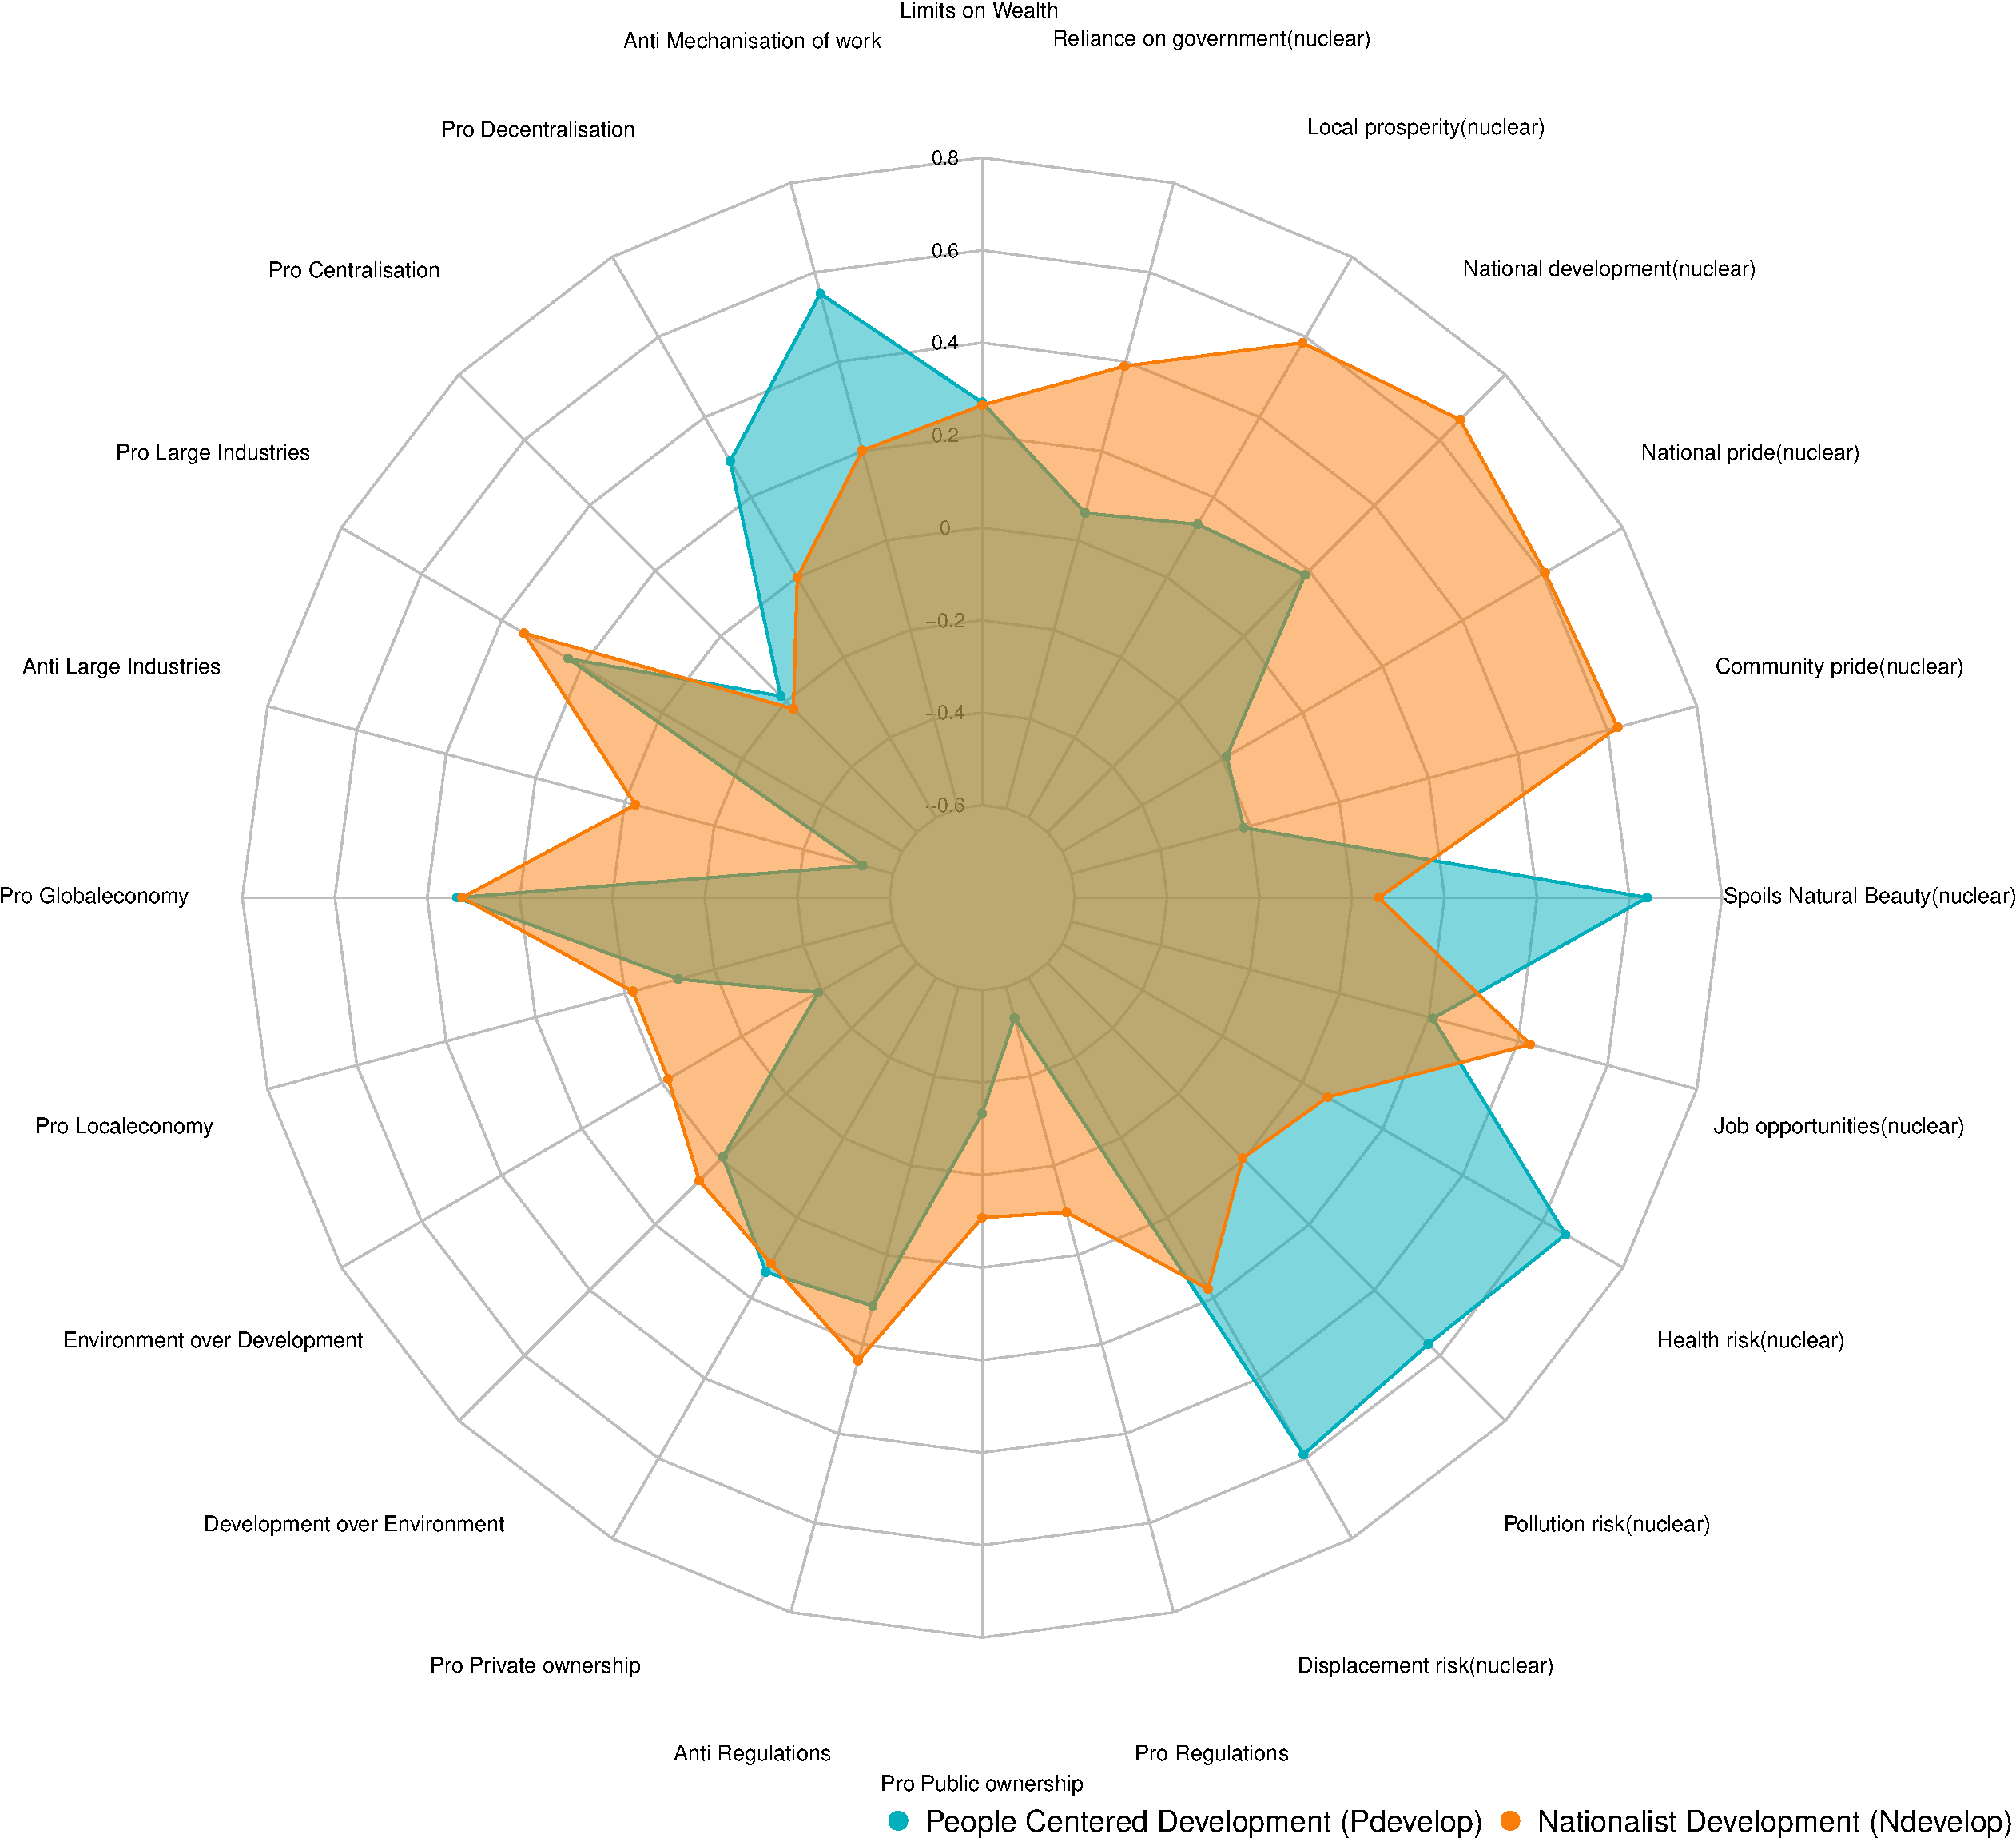
\includegraphics[width=1\linewidth,height=1\textheight]{Paper1_files/figure-latex/unnamed-chunk-22-1}

\newpage

\global\setlength{\Oldarrayrulewidth}{\arrayrulewidth}

\global\setlength{\Oldtabcolsep}{\tabcolsep}

\setlength{\tabcolsep}{0pt}

\renewcommand*{\arraystretch}{1.5}



\providecommand{\ascline}[3]{\noalign{\global\arrayrulewidth #1}\arrayrulecolor[HTML]{#2}\cline{#3}}

\begin{longtable}[c]{cccccc}

\caption{Eco-Pol\ Values\ Factor\ Analysis\ Table}\\

\ascline{1.5pt}{666666}{1-6}

\multicolumn{1}{>{}l}{\textcolor[HTML]{000000}{\fontsize{10}{10}\selectfont{Items}}} & \multicolumn{1}{>{}l}{\textcolor[HTML]{000000}{\fontsize{10}{10}\selectfont{Pdevelop}}} & \multicolumn{1}{>{}l}{\textcolor[HTML]{000000}{\fontsize{10}{10}\selectfont{Ndevelop}}} & \multicolumn{1}{>{}r}{\textcolor[HTML]{000000}{\fontsize{10}{10}\selectfont{Communality}}} & \multicolumn{1}{>{}r}{\textcolor[HTML]{000000}{\fontsize{10}{10}\selectfont{Uniqueness}}} & \multicolumn{1}{>{}r}{\textcolor[HTML]{000000}{\fontsize{10}{10}\selectfont{Complexity}}} \\

\ascline{1.5pt}{666666}{1-6}\endfirsthead \caption[]{Eco-Pol\ Values\ Factor\ Analysis\ Table}\\

\ascline{1.5pt}{666666}{1-6}

\multicolumn{1}{>{}l}{\textcolor[HTML]{000000}{\fontsize{10}{10}\selectfont{Items}}} & \multicolumn{1}{>{}l}{\textcolor[HTML]{000000}{\fontsize{10}{10}\selectfont{Pdevelop}}} & \multicolumn{1}{>{}l}{\textcolor[HTML]{000000}{\fontsize{10}{10}\selectfont{Ndevelop}}} & \multicolumn{1}{>{}r}{\textcolor[HTML]{000000}{\fontsize{10}{10}\selectfont{Communality}}} & \multicolumn{1}{>{}r}{\textcolor[HTML]{000000}{\fontsize{10}{10}\selectfont{Uniqueness}}} & \multicolumn{1}{>{}r}{\textcolor[HTML]{000000}{\fontsize{10}{10}\selectfont{Complexity}}} \\

\ascline{1.5pt}{666666}{1-6}\endhead



\multicolumn{1}{>{}l}{\textcolor[HTML]{000000}{\fontsize{10}{10}\selectfont{Health\ risk(nuclear)}}} & \multicolumn{1}{>{}l}{\textcolor[HTML]{000000}{\fontsize{10}{10}\selectfont{0.657}}} & \multicolumn{1}{>{}l}{\textcolor[HTML]{000000}{\fontsize{10}{10}\selectfont{}}} & \multicolumn{1}{>{}r}{\textcolor[HTML]{000000}{\fontsize{10}{10}\selectfont{0.435}}} & \multicolumn{1}{>{}r}{\textcolor[HTML]{000000}{\fontsize{10}{10}\selectfont{0.565}}} & \multicolumn{1}{>{}r}{\textcolor[HTML]{000000}{\fontsize{10}{10}\selectfont{1.018}}} \\





\multicolumn{1}{>{}l}{\textcolor[HTML]{000000}{\fontsize{10}{10}\selectfont{Spoils\ Natural\ Beauty(nuclear)}}} & \multicolumn{1}{>{}l}{\textcolor[HTML]{000000}{\fontsize{10}{10}\selectfont{0.638}}} & \multicolumn{1}{>{}l}{\textcolor[HTML]{000000}{\fontsize{10}{10}\selectfont{}}} & \multicolumn{1}{>{}r}{\textcolor[HTML]{000000}{\fontsize{10}{10}\selectfont{0.410}}} & \multicolumn{1}{>{}r}{\textcolor[HTML]{000000}{\fontsize{10}{10}\selectfont{0.590}}} & \multicolumn{1}{>{}r}{\textcolor[HTML]{000000}{\fontsize{10}{10}\selectfont{1.017}}} \\





\multicolumn{1}{>{}l}{\textcolor[HTML]{000000}{\fontsize{10}{10}\selectfont{Displacement\ risk(nuclear)}}} & \multicolumn{1}{>{}l}{\textcolor[HTML]{000000}{\fontsize{10}{10}\selectfont{0.59}}} & \multicolumn{1}{>{}l}{\textcolor[HTML]{000000}{\fontsize{10}{10}\selectfont{}}} & \multicolumn{1}{>{}r}{\textcolor[HTML]{000000}{\fontsize{10}{10}\selectfont{0.380}}} & \multicolumn{1}{>{}r}{\textcolor[HTML]{000000}{\fontsize{10}{10}\selectfont{0.620}}} & \multicolumn{1}{>{}r}{\textcolor[HTML]{000000}{\fontsize{10}{10}\selectfont{1.178}}} \\





\multicolumn{1}{>{}l}{\textcolor[HTML]{000000}{\fontsize{10}{10}\selectfont{Pollution\ risk(nuclear)}}} & \multicolumn{1}{>{}l}{\textcolor[HTML]{000000}{\fontsize{10}{10}\selectfont{0.565}}} & \multicolumn{1}{>{}l}{\textcolor[HTML]{000000}{\fontsize{10}{10}\selectfont{}}} & \multicolumn{1}{>{}r}{\textcolor[HTML]{000000}{\fontsize{10}{10}\selectfont{0.319}}} & \multicolumn{1}{>{}r}{\textcolor[HTML]{000000}{\fontsize{10}{10}\selectfont{0.681}}} & \multicolumn{1}{>{}r}{\textcolor[HTML]{000000}{\fontsize{10}{10}\selectfont{1.000}}} \\





\multicolumn{1}{>{}l}{\textcolor[HTML]{000000}{\fontsize{10}{10}\selectfont{Anti\ Mechanisation\ of\ work}}} & \multicolumn{1}{>{}l}{\textcolor[HTML]{000000}{\fontsize{10}{10}\selectfont{0.552}}} & \multicolumn{1}{>{}l}{\textcolor[HTML]{000000}{\fontsize{10}{10}\selectfont{}}} & \multicolumn{1}{>{}r}{\textcolor[HTML]{000000}{\fontsize{10}{10}\selectfont{0.345}}} & \multicolumn{1}{>{}r}{\textcolor[HTML]{000000}{\fontsize{10}{10}\selectfont{0.655}}} & \multicolumn{1}{>{}r}{\textcolor[HTML]{000000}{\fontsize{10}{10}\selectfont{1.262}}} \\





\multicolumn{1}{>{}l}{\textcolor[HTML]{000000}{\fontsize{10}{10}\selectfont{Anti\ Large\ Industries}}} & \multicolumn{1}{>{}l}{\textcolor[HTML]{000000}{\fontsize{10}{10}\selectfont{-0.532}}} & \multicolumn{1}{>{}l}{\textcolor[HTML]{000000}{\fontsize{10}{10}\selectfont{}}} & \multicolumn{1}{>{}r}{\textcolor[HTML]{000000}{\fontsize{10}{10}\selectfont{0.284}}} & \multicolumn{1}{>{}r}{\textcolor[HTML]{000000}{\fontsize{10}{10}\selectfont{0.716}}} & \multicolumn{1}{>{}r}{\textcolor[HTML]{000000}{\fontsize{10}{10}\selectfont{1.004}}} \\





\multicolumn{1}{>{}l}{\textcolor[HTML]{000000}{\fontsize{10}{10}\selectfont{Pro\ Regulations}}} & \multicolumn{1}{>{}l}{\textcolor[HTML]{000000}{\fontsize{10}{10}\selectfont{-0.53}}} & \multicolumn{1}{>{}l}{\textcolor[HTML]{000000}{\fontsize{10}{10}\selectfont{}}} & \multicolumn{1}{>{}r}{\textcolor[HTML]{000000}{\fontsize{10}{10}\selectfont{0.290}}} & \multicolumn{1}{>{}r}{\textcolor[HTML]{000000}{\fontsize{10}{10}\selectfont{0.710}}} & \multicolumn{1}{>{}r}{\textcolor[HTML]{000000}{\fontsize{10}{10}\selectfont{1.065}}} \\





\multicolumn{1}{>{}l}{\textcolor[HTML]{000000}{\fontsize{10}{10}\selectfont{Environment\ over\ Development}}} & \multicolumn{1}{>{}l}{\textcolor[HTML]{000000}{\fontsize{10}{10}\selectfont{}}} & \multicolumn{1}{>{}l}{\textcolor[HTML]{000000}{\fontsize{10}{10}\selectfont{}}} & \multicolumn{1}{>{}r}{\textcolor[HTML]{000000}{\fontsize{10}{10}\selectfont{0.153}}} & \multicolumn{1}{>{}r}{\textcolor[HTML]{000000}{\fontsize{10}{10}\selectfont{0.847}}} & \multicolumn{1}{>{}r}{\textcolor[HTML]{000000}{\fontsize{10}{10}\selectfont{1.003}}} \\





\multicolumn{1}{>{}l}{\textcolor[HTML]{000000}{\fontsize{10}{10}\selectfont{Pro\ Globaleconomy}}} & \multicolumn{1}{>{}l}{\textcolor[HTML]{000000}{\fontsize{10}{10}\selectfont{}}} & \multicolumn{1}{>{}l}{\textcolor[HTML]{000000}{\fontsize{10}{10}\selectfont{}}} & \multicolumn{1}{>{}r}{\textcolor[HTML]{000000}{\fontsize{10}{10}\selectfont{0.218}}} & \multicolumn{1}{>{}r}{\textcolor[HTML]{000000}{\fontsize{10}{10}\selectfont{0.782}}} & \multicolumn{1}{>{}r}{\textcolor[HTML]{000000}{\fontsize{10}{10}\selectfont{1.998}}} \\





\multicolumn{1}{>{}l}{\textcolor[HTML]{000000}{\fontsize{10}{10}\selectfont{Pro\ Public\ ownership}}} & \multicolumn{1}{>{}l}{\textcolor[HTML]{000000}{\fontsize{10}{10}\selectfont{}}} & \multicolumn{1}{>{}l}{\textcolor[HTML]{000000}{\fontsize{10}{10}\selectfont{}}} & \multicolumn{1}{>{}r}{\textcolor[HTML]{000000}{\fontsize{10}{10}\selectfont{0.123}}} & \multicolumn{1}{>{}r}{\textcolor[HTML]{000000}{\fontsize{10}{10}\selectfont{0.877}}} & \multicolumn{1}{>{}r}{\textcolor[HTML]{000000}{\fontsize{10}{10}\selectfont{1.208}}} \\





\multicolumn{1}{>{}l}{\textcolor[HTML]{000000}{\fontsize{10}{10}\selectfont{Pro\ Decentralisation}}} & \multicolumn{1}{>{}l}{\textcolor[HTML]{000000}{\fontsize{10}{10}\selectfont{}}} & \multicolumn{1}{>{}l}{\textcolor[HTML]{000000}{\fontsize{10}{10}\selectfont{}}} & \multicolumn{1}{>{}r}{\textcolor[HTML]{000000}{\fontsize{10}{10}\selectfont{0.084}}} & \multicolumn{1}{>{}r}{\textcolor[HTML]{000000}{\fontsize{10}{10}\selectfont{0.916}}} & \multicolumn{1}{>{}r}{\textcolor[HTML]{000000}{\fontsize{10}{10}\selectfont{1.000}}} \\





\multicolumn{1}{>{}l}{\textcolor[HTML]{000000}{\fontsize{10}{10}\selectfont{Limits\ on\ Wealth}}} & \multicolumn{1}{>{}l}{\textcolor[HTML]{000000}{\fontsize{10}{10}\selectfont{}}} & \multicolumn{1}{>{}l}{\textcolor[HTML]{000000}{\fontsize{10}{10}\selectfont{}}} & \multicolumn{1}{>{}r}{\textcolor[HTML]{000000}{\fontsize{10}{10}\selectfont{0.144}}} & \multicolumn{1}{>{}r}{\textcolor[HTML]{000000}{\fontsize{10}{10}\selectfont{0.856}}} & \multicolumn{1}{>{}r}{\textcolor[HTML]{000000}{\fontsize{10}{10}\selectfont{1.999}}} \\





\multicolumn{1}{>{}l}{\textcolor[HTML]{000000}{\fontsize{10}{10}\selectfont{Pro\ Private\ ownership}}} & \multicolumn{1}{>{}l}{\textcolor[HTML]{000000}{\fontsize{10}{10}\selectfont{}}} & \multicolumn{1}{>{}l}{\textcolor[HTML]{000000}{\fontsize{10}{10}\selectfont{}}} & \multicolumn{1}{>{}r}{\textcolor[HTML]{000000}{\fontsize{10}{10}\selectfont{0.031}}} & \multicolumn{1}{>{}r}{\textcolor[HTML]{000000}{\fontsize{10}{10}\selectfont{0.969}}} & \multicolumn{1}{>{}r}{\textcolor[HTML]{000000}{\fontsize{10}{10}\selectfont{1.943}}} \\





\multicolumn{1}{>{}l}{\textcolor[HTML]{000000}{\fontsize{10}{10}\selectfont{Pro\ Localeconomy}}} & \multicolumn{1}{>{}l}{\textcolor[HTML]{000000}{\fontsize{10}{10}\selectfont{}}} & \multicolumn{1}{>{}l}{\textcolor[HTML]{000000}{\fontsize{10}{10}\selectfont{}}} & \multicolumn{1}{>{}r}{\textcolor[HTML]{000000}{\fontsize{10}{10}\selectfont{0.015}}} & \multicolumn{1}{>{}r}{\textcolor[HTML]{000000}{\fontsize{10}{10}\selectfont{0.985}}} & \multicolumn{1}{>{}r}{\textcolor[HTML]{000000}{\fontsize{10}{10}\selectfont{1.043}}} \\





\multicolumn{1}{>{}l}{\textcolor[HTML]{000000}{\fontsize{10}{10}\selectfont{National\ development(nuclear)}}} & \multicolumn{1}{>{}l}{\textcolor[HTML]{000000}{\fontsize{10}{10}\selectfont{}}} & \multicolumn{1}{>{}l}{\textcolor[HTML]{000000}{\fontsize{10}{10}\selectfont{0.662}}} & \multicolumn{1}{>{}r}{\textcolor[HTML]{000000}{\fontsize{10}{10}\selectfont{0.473}}} & \multicolumn{1}{>{}r}{\textcolor[HTML]{000000}{\fontsize{10}{10}\selectfont{0.527}}} & \multicolumn{1}{>{}r}{\textcolor[HTML]{000000}{\fontsize{10}{10}\selectfont{1.159}}} \\





\multicolumn{1}{>{}l}{\textcolor[HTML]{000000}{\fontsize{10}{10}\selectfont{Community\ pride(nuclear)}}} & \multicolumn{1}{>{}l}{\textcolor[HTML]{000000}{\fontsize{10}{10}\selectfont{}}} & \multicolumn{1}{>{}l}{\textcolor[HTML]{000000}{\fontsize{10}{10}\selectfont{0.623}}} & \multicolumn{1}{>{}r}{\textcolor[HTML]{000000}{\fontsize{10}{10}\selectfont{0.434}}} & \multicolumn{1}{>{}r}{\textcolor[HTML]{000000}{\fontsize{10}{10}\selectfont{0.566}}} & \multicolumn{1}{>{}r}{\textcolor[HTML]{000000}{\fontsize{10}{10}\selectfont{1.234}}} \\





\multicolumn{1}{>{}l}{\textcolor[HTML]{000000}{\fontsize{10}{10}\selectfont{National\ pride(nuclear)}}} & \multicolumn{1}{>{}l}{\textcolor[HTML]{000000}{\fontsize{10}{10}\selectfont{}}} & \multicolumn{1}{>{}l}{\textcolor[HTML]{000000}{\fontsize{10}{10}\selectfont{0.605}}} & \multicolumn{1}{>{}r}{\textcolor[HTML]{000000}{\fontsize{10}{10}\selectfont{0.402}}} & \multicolumn{1}{>{}r}{\textcolor[HTML]{000000}{\fontsize{10}{10}\selectfont{0.598}}} & \multicolumn{1}{>{}r}{\textcolor[HTML]{000000}{\fontsize{10}{10}\selectfont{1.193}}} \\





\multicolumn{1}{>{}l}{\textcolor[HTML]{000000}{\fontsize{10}{10}\selectfont{Local\ prosperity(nuclear)}}} & \multicolumn{1}{>{}l}{\textcolor[HTML]{000000}{\fontsize{10}{10}\selectfont{}}} & \multicolumn{1}{>{}l}{\textcolor[HTML]{000000}{\fontsize{10}{10}\selectfont{0.586}}} & \multicolumn{1}{>{}r}{\textcolor[HTML]{000000}{\fontsize{10}{10}\selectfont{0.360}}} & \multicolumn{1}{>{}r}{\textcolor[HTML]{000000}{\fontsize{10}{10}\selectfont{0.640}}} & \multicolumn{1}{>{}r}{\textcolor[HTML]{000000}{\fontsize{10}{10}\selectfont{1.101}}} \\





\multicolumn{1}{>{}l}{\textcolor[HTML]{000000}{\fontsize{10}{10}\selectfont{Job\ opportunities(nuclear)}}} & \multicolumn{1}{>{}l}{\textcolor[HTML]{000000}{\fontsize{10}{10}\selectfont{}}} & \multicolumn{1}{>{}l}{\textcolor[HTML]{000000}{\fontsize{10}{10}\selectfont{0.427}}} & \multicolumn{1}{>{}r}{\textcolor[HTML]{000000}{\fontsize{10}{10}\selectfont{0.226}}} & \multicolumn{1}{>{}r}{\textcolor[HTML]{000000}{\fontsize{10}{10}\selectfont{0.774}}} & \multicolumn{1}{>{}r}{\textcolor[HTML]{000000}{\fontsize{10}{10}\selectfont{1.453}}} \\





\multicolumn{1}{>{}l}{\textcolor[HTML]{000000}{\fontsize{10}{10}\selectfont{Reliance\ on\ government(nuclear)}}} & \multicolumn{1}{>{}l}{\textcolor[HTML]{000000}{\fontsize{10}{10}\selectfont{}}} & \multicolumn{1}{>{}l}{\textcolor[HTML]{000000}{\fontsize{10}{10}\selectfont{}}} & \multicolumn{1}{>{}r}{\textcolor[HTML]{000000}{\fontsize{10}{10}\selectfont{0.156}}} & \multicolumn{1}{>{}r}{\textcolor[HTML]{000000}{\fontsize{10}{10}\selectfont{0.844}}} & \multicolumn{1}{>{}r}{\textcolor[HTML]{000000}{\fontsize{10}{10}\selectfont{1.049}}} \\





\multicolumn{1}{>{}l}{\textcolor[HTML]{000000}{\fontsize{10}{10}\selectfont{Pro\ Large\ Industries}}} & \multicolumn{1}{>{}l}{\textcolor[HTML]{000000}{\fontsize{10}{10}\selectfont{}}} & \multicolumn{1}{>{}l}{\textcolor[HTML]{000000}{\fontsize{10}{10}\selectfont{}}} & \multicolumn{1}{>{}r}{\textcolor[HTML]{000000}{\fontsize{10}{10}\selectfont{0.173}}} & \multicolumn{1}{>{}r}{\textcolor[HTML]{000000}{\fontsize{10}{10}\selectfont{0.827}}} & \multicolumn{1}{>{}r}{\textcolor[HTML]{000000}{\fontsize{10}{10}\selectfont{1.758}}} \\





\multicolumn{1}{>{}l}{\textcolor[HTML]{000000}{\fontsize{10}{10}\selectfont{Anti\ Regulations}}} & \multicolumn{1}{>{}l}{\textcolor[HTML]{000000}{\fontsize{10}{10}\selectfont{}}} & \multicolumn{1}{>{}l}{\textcolor[HTML]{000000}{\fontsize{10}{10}\selectfont{}}} & \multicolumn{1}{>{}r}{\textcolor[HTML]{000000}{\fontsize{10}{10}\selectfont{0.069}}} & \multicolumn{1}{>{}r}{\textcolor[HTML]{000000}{\fontsize{10}{10}\selectfont{0.931}}} & \multicolumn{1}{>{}r}{\textcolor[HTML]{000000}{\fontsize{10}{10}\selectfont{1.440}}} \\





\multicolumn{1}{>{}l}{\textcolor[HTML]{000000}{\fontsize{10}{10}\selectfont{Pro\ Centralisation}}} & \multicolumn{1}{>{}l}{\textcolor[HTML]{000000}{\fontsize{10}{10}\selectfont{}}} & \multicolumn{1}{>{}l}{\textcolor[HTML]{000000}{\fontsize{10}{10}\selectfont{}}} & \multicolumn{1}{>{}r}{\textcolor[HTML]{000000}{\fontsize{10}{10}\selectfont{0.083}}} & \multicolumn{1}{>{}r}{\textcolor[HTML]{000000}{\fontsize{10}{10}\selectfont{0.917}}} & \multicolumn{1}{>{}r}{\textcolor[HTML]{000000}{\fontsize{10}{10}\selectfont{1.930}}} \\





\multicolumn{1}{>{}l}{\textcolor[HTML]{000000}{\fontsize{10}{10}\selectfont{Development\ over\ Environment}}} & \multicolumn{1}{>{}l}{\textcolor[HTML]{000000}{\fontsize{10}{10}\selectfont{}}} & \multicolumn{1}{>{}l}{\textcolor[HTML]{000000}{\fontsize{10}{10}\selectfont{}}} & \multicolumn{1}{>{}r}{\textcolor[HTML]{000000}{\fontsize{10}{10}\selectfont{0.004}}} & \multicolumn{1}{>{}r}{\textcolor[HTML]{000000}{\fontsize{10}{10}\selectfont{0.996}}} & \multicolumn{1}{>{}r}{\textcolor[HTML]{000000}{\fontsize{10}{10}\selectfont{1.025}}} \\

\ascline{1.5pt}{666666}{1-6}



\end{longtable}



\arrayrulecolor[HTML]{000000}

\global\setlength{\arrayrulewidth}{\Oldarrayrulewidth}

\global\setlength{\tabcolsep}{\Oldtabcolsep}

\renewcommand*{\arraystretch}{1}

\global\setlength{\Oldarrayrulewidth}{\arrayrulewidth}

\global\setlength{\Oldtabcolsep}{\tabcolsep}

\setlength{\tabcolsep}{0pt}

\renewcommand*{\arraystretch}{1.5}



\providecommand{\ascline}[3]{\noalign{\global\arrayrulewidth #1}\arrayrulecolor[HTML]{#2}\cline{#3}}

\begin{longtable}[c]{ccc}

\caption{Eigenvalues\ and\ Variance\ Explained\ for\ Rotated\ Factor\ Solution}\\

\ascline{1.5pt}{666666}{1-3}

\multicolumn{1}{>{}l}{\textcolor[HTML]{000000}{\fontsize{10}{10}\selectfont{Property}}} & \multicolumn{1}{>{}r}{\textcolor[HTML]{000000}{\fontsize{10}{10}\selectfont{Pdevelop}}} & \multicolumn{1}{>{}r}{\textcolor[HTML]{000000}{\fontsize{10}{10}\selectfont{Ndevelop}}} \\

\ascline{1.5pt}{666666}{1-3}\endfirsthead \caption[]{Eigenvalues\ and\ Variance\ Explained\ for\ Rotated\ Factor\ Solution}\\

\ascline{1.5pt}{666666}{1-3}

\multicolumn{1}{>{}l}{\textcolor[HTML]{000000}{\fontsize{10}{10}\selectfont{Property}}} & \multicolumn{1}{>{}r}{\textcolor[HTML]{000000}{\fontsize{10}{10}\selectfont{Pdevelop}}} & \multicolumn{1}{>{}r}{\textcolor[HTML]{000000}{\fontsize{10}{10}\selectfont{Ndevelop}}} \\

\ascline{1.5pt}{666666}{1-3}\endhead



\multicolumn{1}{>{}l}{\textcolor[HTML]{000000}{\fontsize{10}{10}\selectfont{SS\ loadings}}} & \multicolumn{1}{>{}r}{\textcolor[HTML]{000000}{\fontsize{10}{10}\selectfont{3.224}}} & \multicolumn{1}{>{}r}{\textcolor[HTML]{000000}{\fontsize{10}{10}\selectfont{2.388}}} \\





\multicolumn{1}{>{}l}{\textcolor[HTML]{000000}{\fontsize{10}{10}\selectfont{Proportion\ Var}}} & \multicolumn{1}{>{}r}{\textcolor[HTML]{000000}{\fontsize{10}{10}\selectfont{0.134}}} & \multicolumn{1}{>{}r}{\textcolor[HTML]{000000}{\fontsize{10}{10}\selectfont{0.099}}} \\





\multicolumn{1}{>{}l}{\textcolor[HTML]{000000}{\fontsize{10}{10}\selectfont{Cumulative\ Var}}} & \multicolumn{1}{>{}r}{\textcolor[HTML]{000000}{\fontsize{10}{10}\selectfont{0.134}}} & \multicolumn{1}{>{}r}{\textcolor[HTML]{000000}{\fontsize{10}{10}\selectfont{0.234}}} \\





\multicolumn{1}{>{}l}{\textcolor[HTML]{000000}{\fontsize{10}{10}\selectfont{Proportion\ Explained}}} & \multicolumn{1}{>{}r}{\textcolor[HTML]{000000}{\fontsize{10}{10}\selectfont{0.575}}} & \multicolumn{1}{>{}r}{\textcolor[HTML]{000000}{\fontsize{10}{10}\selectfont{0.425}}} \\





\multicolumn{1}{>{}l}{\textcolor[HTML]{000000}{\fontsize{10}{10}\selectfont{Cumulative\ Proportion}}} & \multicolumn{1}{>{}r}{\textcolor[HTML]{000000}{\fontsize{10}{10}\selectfont{0.575}}} & \multicolumn{1}{>{}r}{\textcolor[HTML]{000000}{\fontsize{10}{10}\selectfont{1.000}}} \\

\ascline{1.5pt}{666666}{1-3}



\end{longtable}



\arrayrulecolor[HTML]{000000}

\global\setlength{\arrayrulewidth}{\Oldarrayrulewidth}

\global\setlength{\tabcolsep}{\Oldtabcolsep}

\renewcommand*{\arraystretch}{1}

\newpage

\begin{landscape}
\begin{longtable}[t]{>{\raggedright\arraybackslash}p{4cm}>{\raggedright\arraybackslash}p{4cm}>{\raggedright\arraybackslash}p{9cm}ll}
\caption{\label{tab:unnamed-chunk-27}Two Factor Solution: Economic and Political Values Scale}\\
\toprule
Scale & Code & Items and Loadings & Alpha & Variance\\
\midrule
\endfirsthead
\caption[]{Two Factor Solution: Economic and Political Values Scale \textit{(continued)}}\\
\toprule
Scale & Code & Items and Loadings & Alpha & Variance\\
\midrule
\endhead

\endfoot
\bottomrule
\endlastfoot
\cellcolor{gray!6}{People Centered Development (Pdevelop)} & \cellcolor{gray!6}{Health risk(nuclear)} & \cellcolor{gray!6}{Nuclear energy poses a great risk to the health of people living around it.(0.657)} & \cellcolor{gray!6}{0.757} & \cellcolor{gray!6}{}\\
 & Spoils Natural Beauty(nuclear) & Nuclear energy spoils the natural beauty of the landscape.(0.638) &  & \\
\cellcolor{gray!6}{} & \cellcolor{gray!6}{Anti Mechanisation of work} & \cellcolor{gray!6}{Rapid mechanization of work is taking away jobs from workers in this country.(0.552)} & \cellcolor{gray!6}{} & \cellcolor{gray!6}{}\\
 & Anti Large Industries & Large corporations are destroying the local industries in India and benefiting only a handful of people.(-0.532) &  & \\
\cellcolor{gray!6}{} & \cellcolor{gray!6}{Displacement risk(nuclear)} & \cellcolor{gray!6}{Nuclear energy is leading to displacement of people from their land.(0.59)} & \cellcolor{gray!6}{} & \cellcolor{gray!6}{}\\
\addlinespace
 & Pollution risk(nuclear) & Nuclear energy increases pollution of air/water/land.(0.565) &  & \\
\cellcolor{gray!6}{} & \cellcolor{gray!6}{Pro Regulations} & \cellcolor{gray!6}{Regardless of ownership, the government should pass strong regulations and implement them.(-0.53)} & \cellcolor{gray!6}{} & \cellcolor{gray!6}{}\\
Nationalist Development (Ndevelop) & National development(nuclear) & Nuclear energy pushes forward the country's development.(0.662) & 0.725 & \\
\cellcolor{gray!6}{} & \cellcolor{gray!6}{Community pride(nuclear)} & \cellcolor{gray!6}{I would be proud if my community used nuclear energy.(0.623)} & \cellcolor{gray!6}{} & \cellcolor{gray!6}{}\\
 & National pride(nuclear) & Nuclear energy is a mark of pride for our nation.(0.605) &  & \\
\addlinespace
\cellcolor{gray!6}{} & \cellcolor{gray!6}{Local prosperity(nuclear)} & \cellcolor{gray!6}{Nuclear energy brings economic prosperity to the surrounding regions.(0.586)} & \cellcolor{gray!6}{} & \cellcolor{gray!6}{}\\
 & Job opportunities(nuclear) & Nuclear energy will bring jobs to the local community.(0.427) &  & \\*
\end{longtable}
\end{landscape}

\newpage

\hypertarget{h4-economic-and-political-values-will-be-important-in-explaining-perceived-risk-from-nuclear-energy}{%
\section{H4 : Economic and Political Values will be important in
explaining perceived risk from Nuclear
Energy}\label{h4-economic-and-political-values-will-be-important-in-explaining-perceived-risk-from-nuclear-energy}}

\begingroup\setlength{\tabcolsep}{1pt}

\renewcommand{\arraystretch}{0.7}

\% Table created by stargazer v.5.2.3 by Marek Hlavac, Social Policy
Institute. E-mail: marek.hlavac at gmail.com \% Date and time: Mon, Sep
18, 2023 - 18:52:04

\begin{table}[!htbp] \centering 
  \caption{Results from 2 linear regression models} 
  \label{} 
\begin{tabular}{@{\extracolsep{5pt}}lcc} 
\\[-1.8ex]\hline 
\hline \\[-1.8ex] 
 & \multicolumn{2}{c}{\textit{Dependent variable:}} \\ 
\cline{2-3} 
\\[-1.8ex] & \multicolumn{2}{c}{Risky\_Nuclear} \\ 
\\[-1.8ex] & (1) & (2)\\ 
\hline \\[-1.8ex] 
 Uppercaste & $-$0.029 & $-$0.035 \\ 
  & (0.107) & (0.105) \\ 
  & & \\ 
 Male & $-$0.102 & $-$0.085 \\ 
  & (0.117) & (0.116) \\ 
  & & \\ 
 Hindu & $-$0.025 & 0.025 \\ 
  & (0.118) & (0.117) \\ 
  & & \\ 
 UrbanUrban & $-$0.003 & 0.021 \\ 
  & (0.112) & (0.111) \\ 
  & & \\ 
 age & 0.050 & 0.036 \\ 
  & (0.052) & (0.051) \\ 
  & & \\ 
 StateRajasthan & 0.445$^{***}$ & 0.186 \\ 
  & (0.169) & (0.181) \\ 
  & & \\ 
 StateTamil Nadu & 1.141$^{***}$ & 1.282$^{***}$ \\ 
  & (0.197) & (0.240) \\ 
  & & \\ 
 StateUttar Pradesh & $-$0.006 & $-$0.061 \\ 
  & (0.192) & (0.193) \\ 
  & & \\ 
 StateWest Bengal & 1.120$^{***}$ & 0.965$^{***}$ \\ 
  & (0.216) & (0.226) \\ 
  & & \\ 
 KahanS & $-$0.202$^{*}$ & $-$0.120 \\ 
  & (0.110) & (0.111) \\ 
  & & \\ 
 KahanH & 0.077 & $-$0.012 \\ 
  & (0.102) & (0.102) \\ 
  & & \\ 
 Pdevelop &  & 0.159$^{**}$ \\ 
  &  & (0.075) \\ 
  & & \\ 
 Ndevelop &  & 0.230$^{***}$ \\ 
  &  & (0.061) \\ 
  & & \\ 
 Constant & 3.008$^{***}$ & 3.033$^{***}$ \\ 
  & (0.173) & (0.172) \\ 
  & & \\ 
\hline \\[-1.8ex] 
Observations & 405 & 405 \\ 
R$^{2}$ & 0.260 & 0.290 \\ 
Adjusted R$^{2}$ & 0.240 & 0.267 \\ 
Residual Std. Error & 0.941 (df = 393) & 0.924 (df = 391) \\ 
F Statistic & 12.573$^{***}$ (df = 11; 393) & 12.298$^{***}$ (df = 13; 391) \\ 
\hline 
\hline \\[-1.8ex] 
\textit{Note:}  & \multicolumn{2}{r}{$^{*}$p$<$0.1; $^{**}$p$<$0.05; $^{***}$p$<$0.01} \\ 
\end{tabular} 
\end{table} 
\endgroup

\newpage

\newpage

\hypertarget{appendix-characteristics-of-the-sample}{%
\section{Appendix: Characteristics of the
Sample}\label{appendix-characteristics-of-the-sample}}

The following graph shows that distribution of different demographic
variables in our sample of 2,160 from the combined dataset from both
surveys. The percentages are rounded off to whole numbers.

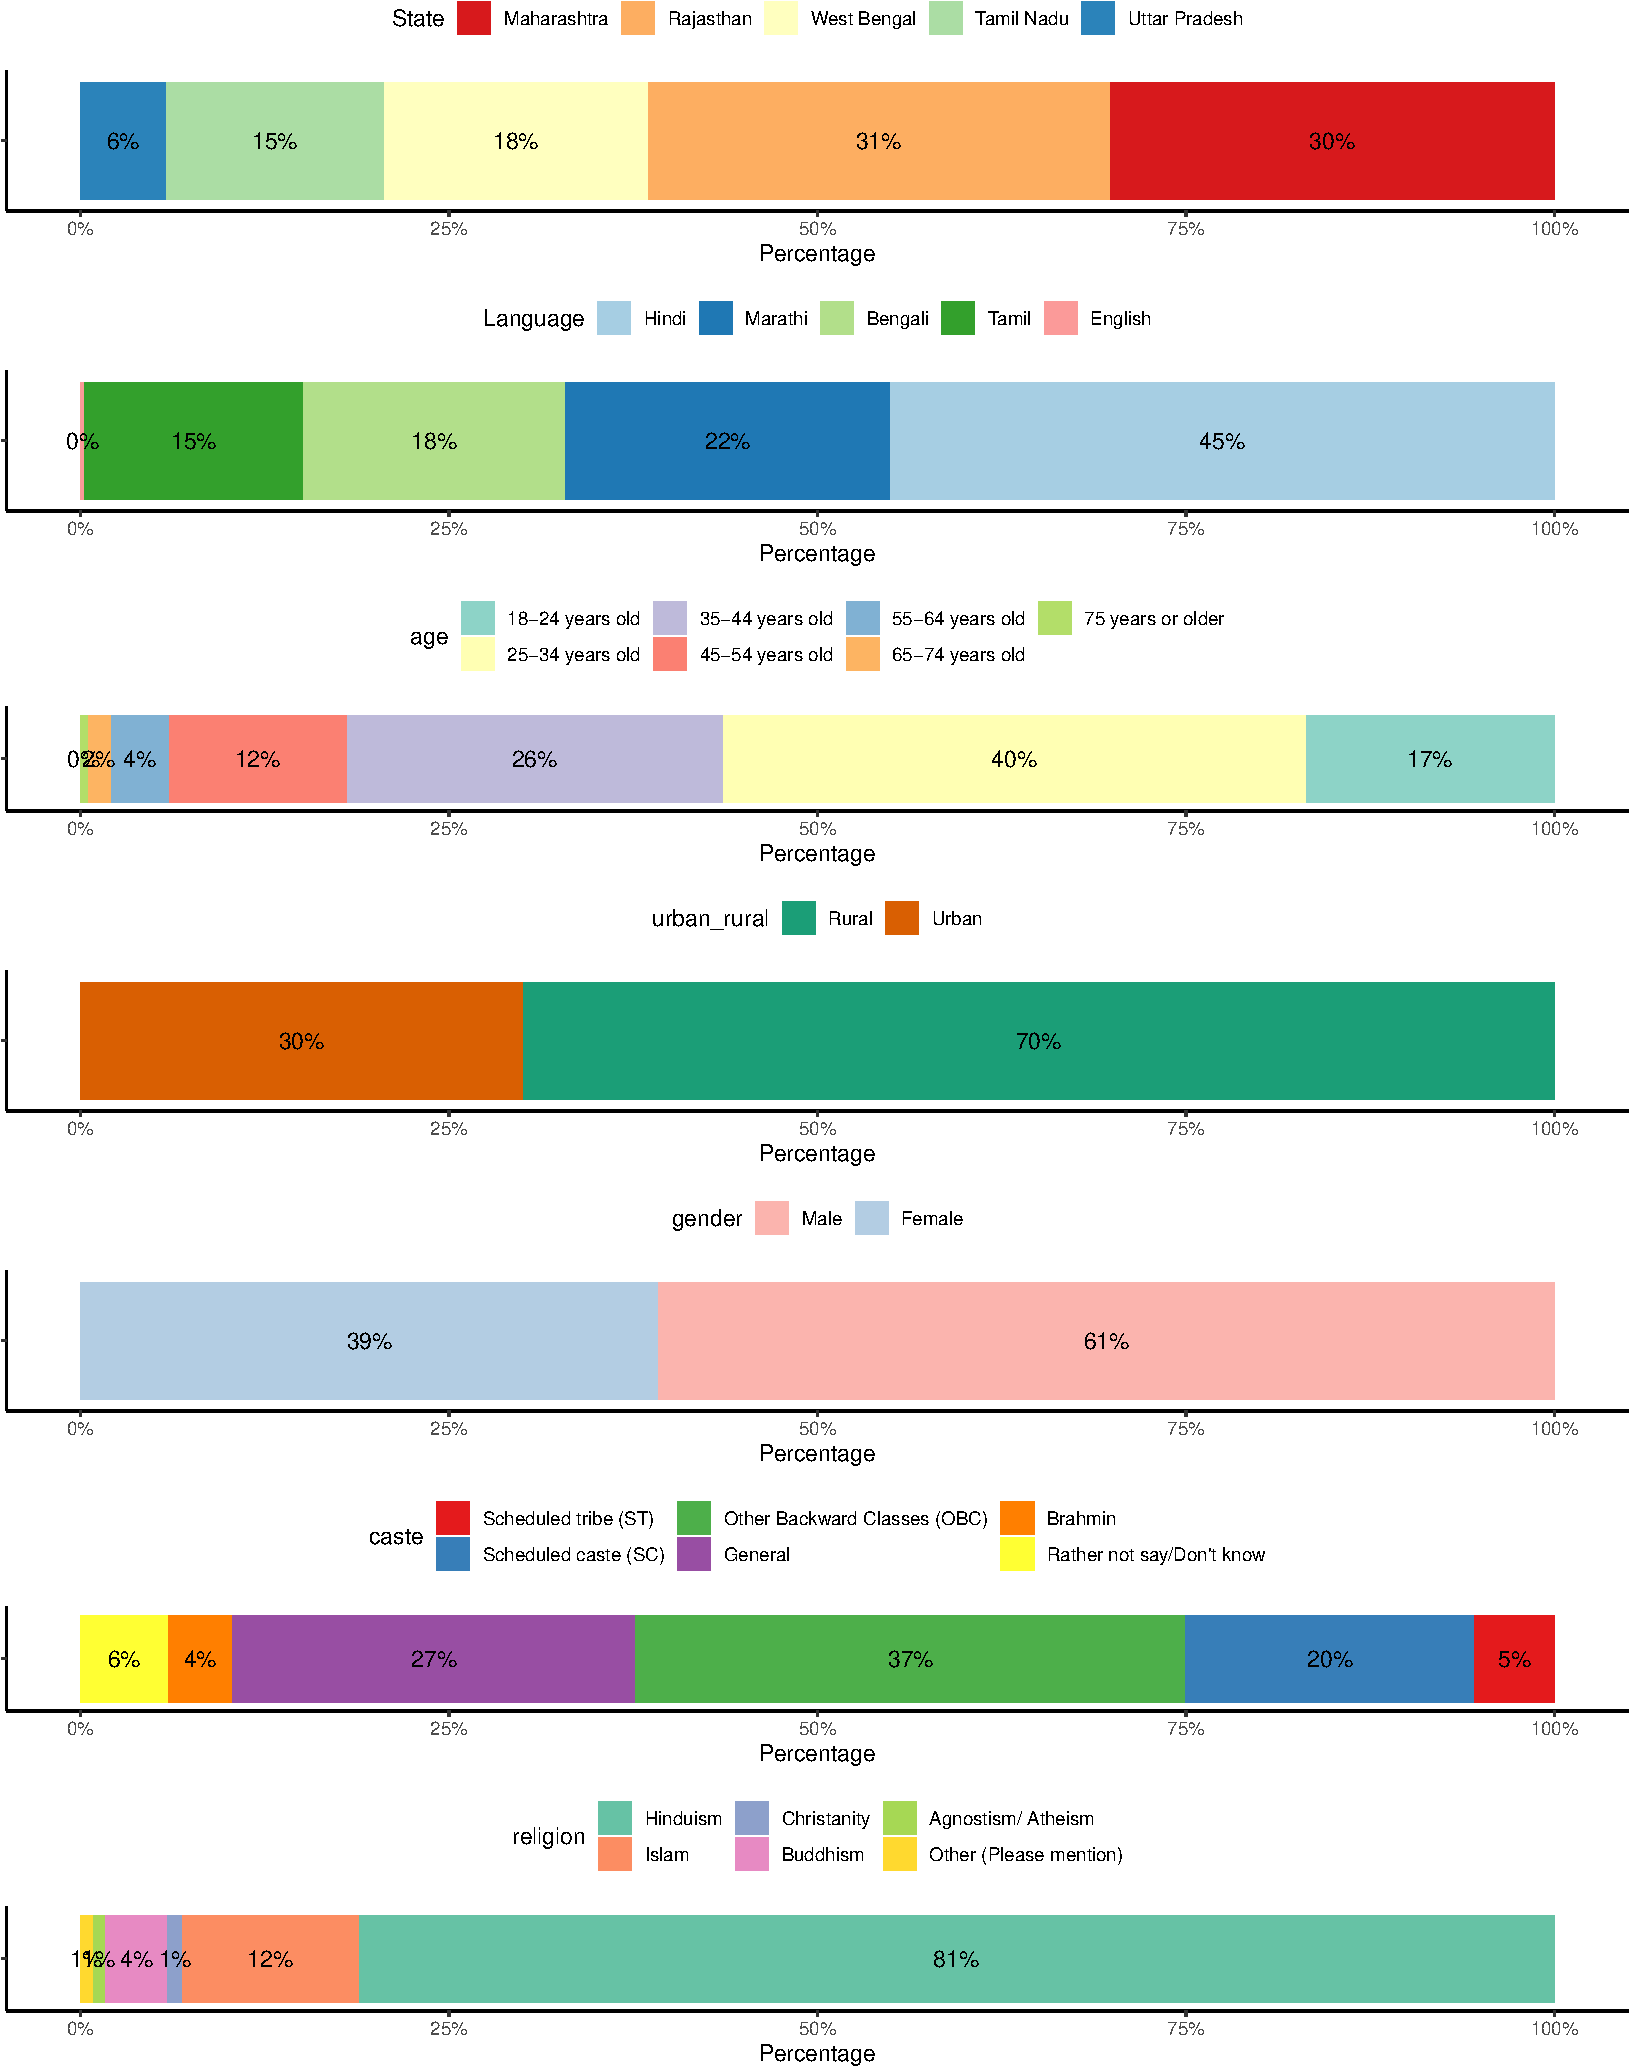
\includegraphics[width=0.8\linewidth,height=0.8\textheight]{Paper1_files/figure-latex/unnamed-chunk-32-1}

\end{document}
